% =====================================================================
%  CAPÍTULO 6 · PRUEBAS Y RESULTADOS
%  Función: demostrar CON EVIDENCIA que se cumplen requisitos y objetivos.
%  Reglas clave:
%   - Casos de prueba con entrada/pasos -> resultado esperado -> obtenido.
%     «Se ha probado manualmente» no es evidencia.
%   - NUNCA presentes como hecho algo propuesto o futuro: si una prueba no
%     se pudo hacer, dilo explícitamente.
%   - Cifras coherentes entre texto, tablas y resumen. Con usuarios:
%     N, perfil, instrumento y valores absolutos («6 de 8», no solo «75 %»).
%   - Cada gráfica se interpreta: qué se ve, qué significa, qué se decide.
%   - Las hipótesis no son hechos («indicios de», no «se confirma»).
% =====================================================================
\chapter{Pruebas y resultados}
\label{cap:pruebas}

Este capítulo presenta la estrategia de pruebas, los resultados obtenidos y su
relación con los requisitos y los objetivos del trabajo.

\section{Estrategia de pruebas}
\label{sec:estrategia}

Se han realizado tres tipos de pruebas: pruebas funcionales de cada requisito,
pruebas de carga para el requisito de rendimiento (RNF-01) y una prueba de
usabilidad con usuarios (RNF-02). Las pruebas funcionales y de carga se
ejecutaron sobre la versión etiquetada \texttt{\tfgversion} del repositorio
(Apéndice~\ref{ap:repositorio}).

\section{Pruebas funcionales}
\label{sec:pruebas-funcionales}

La Tabla~\ref{tab:casos} recoge los casos de prueba de los requisitos
funcionales. Los cuatro casos se superaron; el caso PR-04, que simula dos
reservas simultáneas de la misma sala, confirma que la transacción del
Listado~\ref{lst:reserva} evita el solapamiento.

\begin{table}[htbp]
  \centering
  \caption{Casos de prueba funcionales.}
  \label{tab:casos}
  \small
  \begin{tabularx}{\textwidth}{@{}llLLl@{}}
    \toprule
    \textbf{ID} & \textbf{Req.} & \textbf{Pasos / entrada} & \textbf{Resultado esperado} & \textbf{Estado} \\
    \midrule
    PR-01 & RF-01 & Abrir la app con dos salas libres & Se listan las dos salas & Superada \\
    PR-02 & RF-02 & Reservar la sala A-12 desde el inicio & Reserva creada en 2 pasos & Superada \\
    PR-03 & RF-03 & Reserva a 11 min vista & Aviso a los 10 min & Superada \\
    PR-04 & RF-04 & Dos peticiones simultáneas a la misma franja & Una creada, otra con error 409 & Superada \\
    \bottomrule
  \end{tabularx}
  \fuente{Elaboración propia.}
\end{table}

\section{Pruebas de rendimiento}
\label{sec:rendimiento}

Se midió la latencia media de la \ac{API} con 10 a 400 usuarios concurrentes
simulados, repitiendo cada medida cinco veces. La
Figura~\ref{fig:latencia} compara la versión inicial con la versión que añade
una caché de consultas. Sin caché, la latencia supera el umbral de
\qty{100}{ms} a partir de unos 200 usuarios; con caché, se mantiene por debajo
del umbral en todo el rango medido, con \qty{92}{ms} para 400 usuarios. Por
tanto, RNF-01 se cumple con margen y el objetivo~\ref{obj:rendimiento} se
alcanza.

\begin{figure}[htbp]
  \centering
  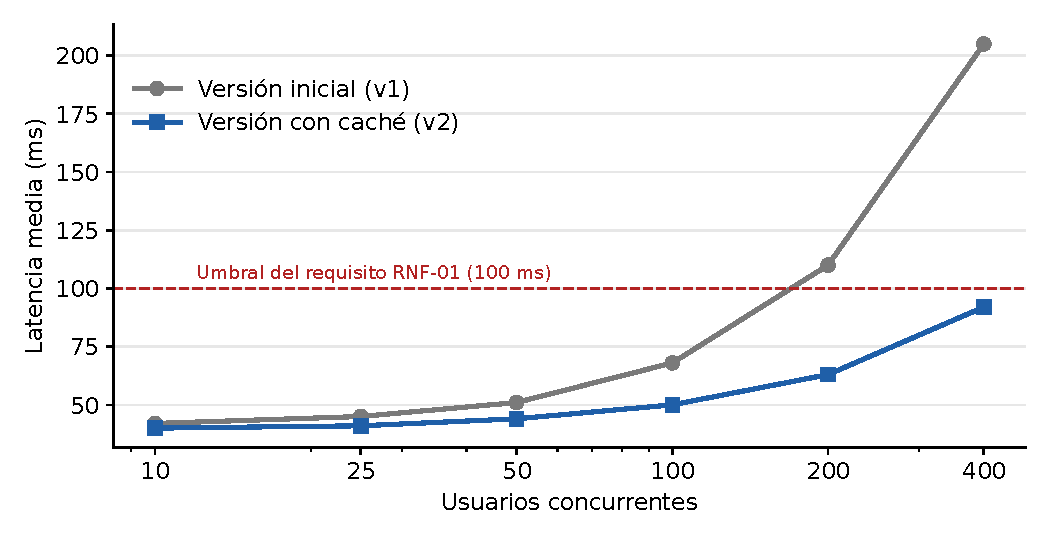
\includegraphics[width=\textwidth]{resultados_latencia}
  \caption{Latencia media de la API según el número de usuarios concurrentes.}
  \label{fig:latencia}
  \fuente{Elaboración propia (datos de ejemplo, ficticios).}
\end{figure}

% GUÍA: las gráficas de datos van a ANCHO COMPLETO, con ejes etiquetados y
% unidades. Expórtalas en vectorial (PDF) desde tu script y guarda el script
% en el repositorio para poder regenerarlas.

\section{Prueba de usabilidad}
\label{sec:usabilidad-resultados}

Ocho estudiantes de grado, sin relación con el proyecto, realizaron tres tareas
de reserva y respondieron después el cuestionario \ac{SUS}
(Ecuación~\ref{eq:sus}). La puntuación media fue de 81 (desviación típica 7),
por encima del umbral de 70 fijado en RNF-02. Siete de los ocho participantes
(88\,\%) completaron todas las tareas sin ayuda; el único error repetido fue no
encontrar el botón de cancelar una reserva, que se movió en el incremento 3.

% GUÍA: si la prueba con usuarios NO se pudo hacer, escríbelo así:
% «La prueba de usabilidad prevista en la planificación no se ha podido
% realizar; se propone como trabajo futuro (Sección 7.3).»

\section{Trazabilidad y resumen de resultados}
\label{sec:trazabilidad}

La Tabla~\ref{tab:trazabilidad} relaciona cada objetivo con los requisitos que
lo concretan y con las pruebas que lo validan, y resume el resultado obtenido.

\begin{table}[htbp]
  \centering
  \caption{Trazabilidad entre objetivos, requisitos y pruebas.}
  \label{tab:trazabilidad}
  \small
  \begin{tabularx}{\textwidth}{@{}llLL@{}}
    \toprule
    \textbf{Objetivo} & \textbf{Requisitos} & \textbf{Evidencia} & \textbf{Resultado} \\
    \midrule
    \ref{obj:estado}      & ---           & Tabla~\ref{tab:comparativa}  & Comparativa de 3 soluciones \\
    \ref{obj:app}         & RF-01 a RF-04 & PR-01 a PR-04 (Tabla~\ref{tab:casos}) & 4/4 pruebas superadas \\
    \ref{obj:rendimiento} & RNF-01        & Figura~\ref{fig:latencia}    & \qty{92}{ms} con 400 usuarios \\
    \ref{obj:validacion}  & RNF-02        & Sección~\ref{sec:usabilidad-resultados} & SUS = 81 ($n = 8$) \\
    \bottomrule
  \end{tabularx}
  \fuente{Elaboración propia.}
\end{table}

\section{Discusión y limitaciones}
\label{sec:discusion}

Interpreta los resultados con espíritu crítico: qué significan, qué no
demuestran y qué podría haber influido. En este ejemplo, las pruebas de carga
se hicieron en un único servidor y con usuarios simulados, y la prueba de
usabilidad tiene una muestra pequeña ($n = 8$), por lo que los resultados son
indicativos y no generalizables a todo el campus.
